\documentclass[final]{beamer}
% \usecolortheme{crane}
\mode<presentation>
{
  \usetheme{I6pd2}
}
\usepackage{times}
\usepackage{amsmath,amssymb}
%\usepackage{sfmath} % for sans serif math fonts; wget http://dtrx.de/od/tex/sfmath.sty
\usepackage[english]{babel}
\usepackage[utf8]{inputenc}
\usepackage[size=a4, scale=0.4]{beamerposter}
\usepackage{booktabs,array}
\usepackage{wrapfig}
% \usepackage{enumitem}

% Display a grid to help align images
% \beamertemplategridbackground[3mm]

\title{\LARGE Algorithmic Analysis of Code-Breaking Games}

\author{Miroslav Klimoš, Prof. RNDr. Antonín Kučera Ph.D.}
\institute[RWTH Aachen University] % (optional, but mostly needed)
{
  Faculty of Informatics, Masaryk University, Brno
}

\date[May. 28th, 2008]{May. 28th, 2008}

\newcommand{\thando}[4]{
\begin{columns}[T]
\begin{column}{\leftmarginii}
\end{column}
\begin{column}{#3\textwidth}
\vspace{-1.5mm}
\begin{itemize}
#1
\end{itemize}
\end{column}
\begin{column}{#4\textwidth}
#2
\end{column}
\end{columns}\medskip}

\begin{document}
\begin{frame}{} 
\begin{columns}[t]
  %%%%%%%%%%%%%%%%%%%%%%%%%%%%%%%%%%%%%%%%%%%%%%%%%%%%%%%%%%%%%%%%%%%%%%%%%%%%%%%%%%%%%%%%%%%%%%%%%%%%
  %%%%%%%%%%%%%%%%%%%%%%%%%%%%%%%%%%%%%%%%%%%%%%%%%%%%%%%%%%%%%%%%%%%%%%%%%%%%%%%%%%%%%%%%%%%%%%%%%%%%
  \begin{column}{.48\linewidth}
    
    \begin{block}{Code-breaking games}
      \begin{itemize}
      \item 2 players: \emph{codemaker} and \emph{codebreaker}
      \item codemaker selects a secret code
      \item codebreaker strives to reveal the code through a series of \emph{experiments} whose outcomes give partial information about the code
      \end{itemize}
    \end{block}
    
    \begin{block}{Example: Mastermind}
    \begin{columns}
      \begin{column}{\parindent}\end{column}
      \begin{column}{.78\textwidth}
        \begin{itemize}
        \item Code: combination of $n$ \emph{coloured pegs}
        \item Codebreaker makes guesses (experiments)
        \item Guesses are evaluated with \emph{black and white markers}
        \item Black marker = correct both color and position
        \item White marker = the color is present at different position
        \end{itemize}
      \end{column}

      \begin{column}{.22\textwidth}
        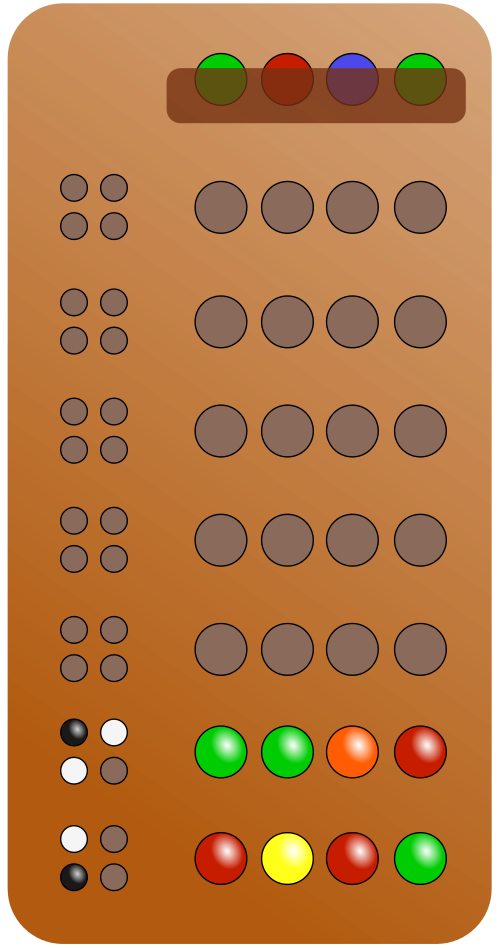
\includegraphics[width=1.8cm]{../pictures/mastermind.png}
      \end{column}
    \end{columns}
    \end{block}
    
    \begin{block}{Example: Counterfeit coin}
    \begin{columns}
      \begin{column}{\parindent}\end{column}
      \begin{column}{.78\textwidth}
      \begin{itemize}
        \item Problem of identifying an odd-weight coin using balance scale
        \item Code: identity of the unique countefeit coin
        \item Codebreaker puts coins on the balance scale and observes the outcome (left pan is lighter / heavier / same)
      \end{itemize}    
      \end{column}
      \begin{column}{.22\textwidth}
        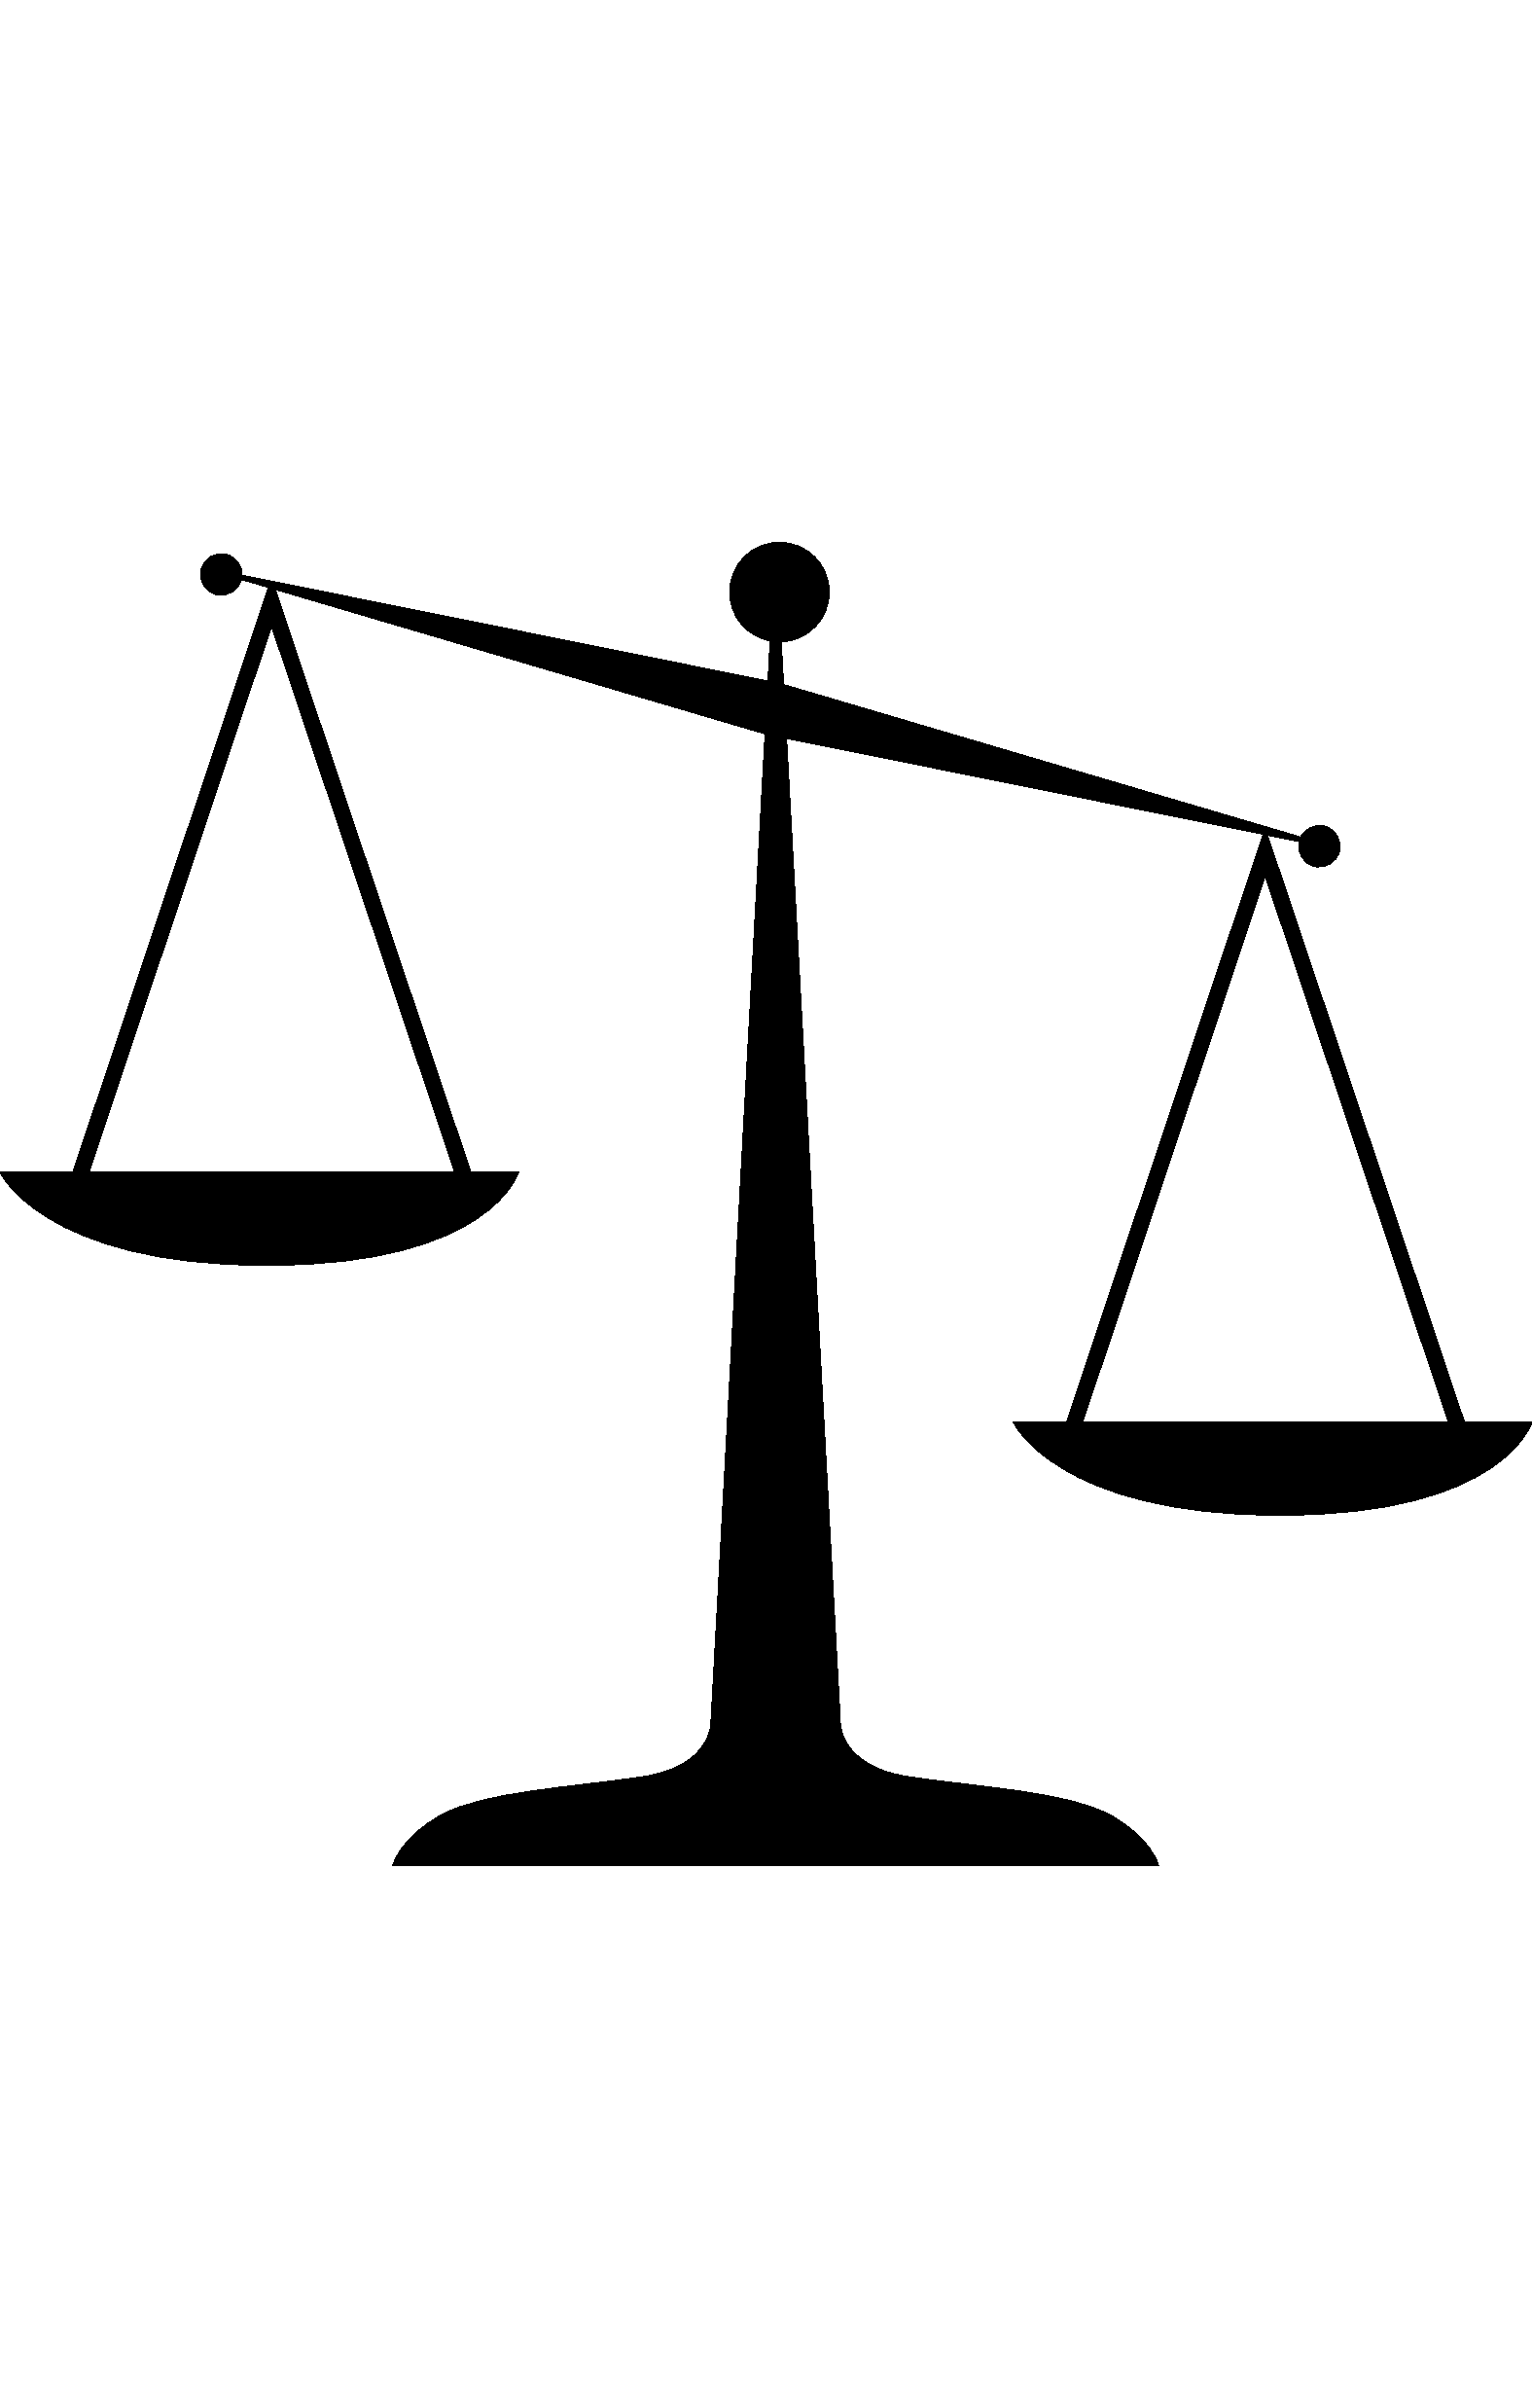
\includegraphics[width=2cm]{../pictures/scales.pdf}
      \end{column}
    \end{columns}
    \end{block}
      
    \begin{block}{Questions and problems}
      \begin{itemize}
      \item How should the codebreaker play in order to minimize the number of experiments needed to undoubtedly determine the code?
      \item Is there a strategy for experiment selection that guarantees revealing the code after at most $k$ experiments?
      \item What strategy is optimal with respect to the average-case number of experiments, given that the code is selected from the given set with uniform distribution?
      \end{itemize}
    \end{block}

  \end{column}
  %%%%%%%%%%%%%%%%%%%%%%%%%%%%%%%%%%%%%%%%%%%%%%%%%%%%%%%%%%%%%%%%%%%%%%%%%%%%%%%%%%%%%%%%%%%%%%%%%%%%
  %%%%%%%%%%%%%%%%%%%%%%%%%%%%%%%%%%%%%%%%%%%%%%%%%%%%%%%%%%%%%%%%%%%%%%%%%%%%%%%%%%%%%%%%%%%%%%%%%%%%
  \begin{column}{.48\linewidth}
    \begin{block}{Challenges and solutions}
      \begin{enumerate}
      \item Create a general, formal model of code breking games
        \thando{
        \item Model based on propositional logic
        \item Secret code = valuation of variables
        \item Partial information = logical formula
        }{
          \hspace{-12mm}
          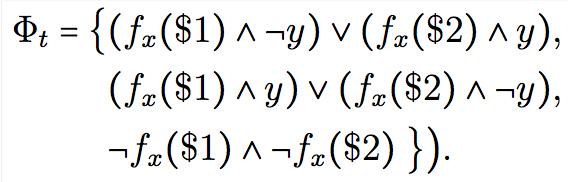
\includegraphics[scale=0.45]{img-model.png}
        }{0.65}{0.35}
      \item Suggest general strategies for experiment selection
        \thando{
        \item \emph{``Select an experiment that minimizes the maximal number of possibilities for the code in the next round''}
        \item Several strategies of this kind are formalized within the~model
        }{
          \hspace{-5mm}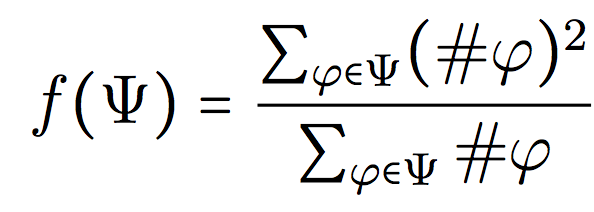
\includegraphics[width=3cm]{img-strategy.png}
        }{0.7}{0.3}
      \item Propose algorithms for strategy evaluation and synthesis
        \thando{
        \item Based on intelligent backtracking
        \item Symmetry detection reduces the size of the state-space
        }{
          \hspace{-10mm}
          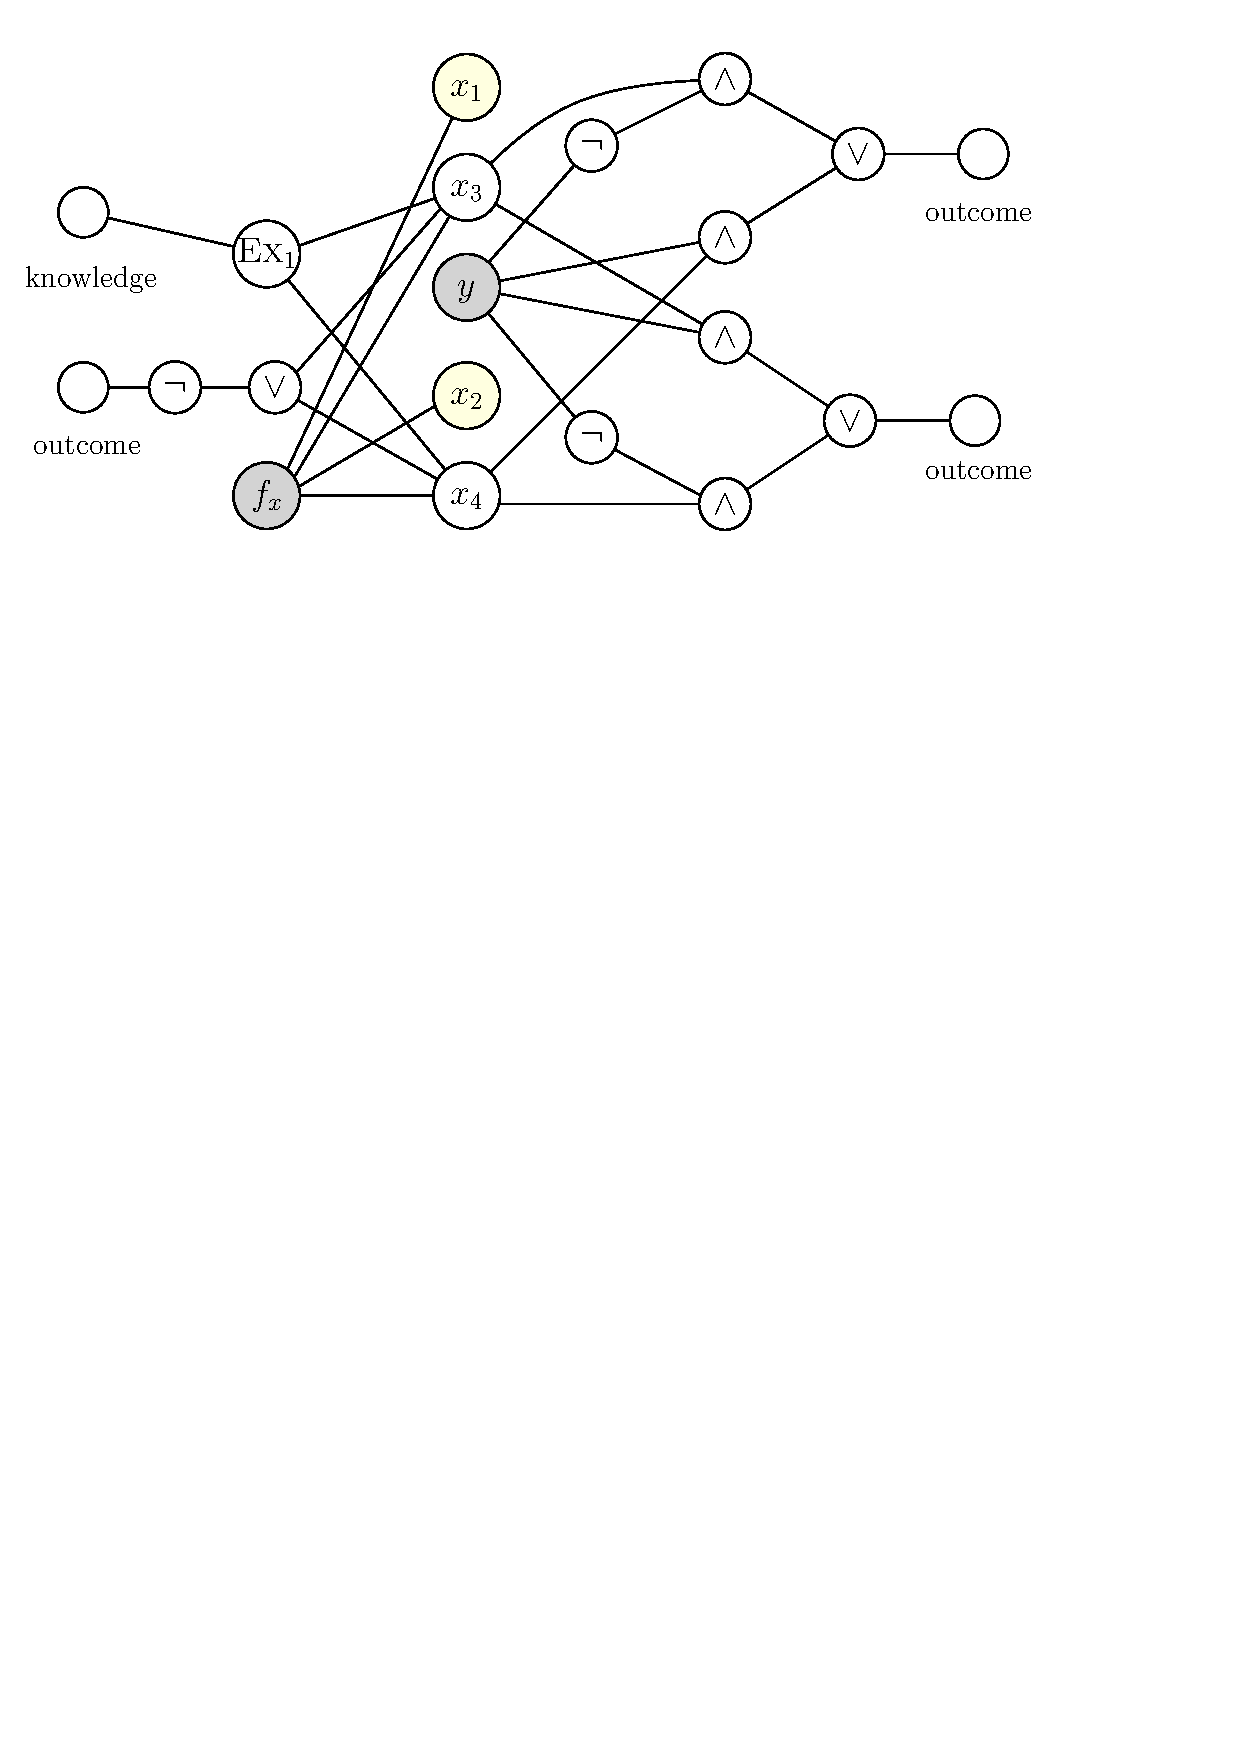
\includegraphics[width=4cm]{../pictures/exp-graph-sim.pdf}
        }{0.65}{0.35}
      \item Design a computer language for game specification
        \thando{
        \item Follows directly from the formal model
        \item Built on top of Python for easier generation
        }{
          \hspace{-22mm}
          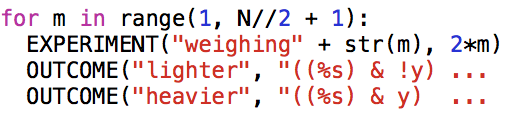
\includegraphics[width=4cm]{img-language.png}
        }{0.75}{0.25}
      \item Implement proposed algorithms in a computer program
        \thando{
        \item Command-line tool COBRA written in C++
        \item Uses modern SAT solvers for satisfiability queries needed by the algorithms
        \item Graph canonization tool Bliss is utilized for symmetry detection
        }{

        }{0.95}{0.05}
      \item Use the tool to create new and reproduce existing results
        \thando{
        \item COBRA can easily reproduce some existing results for~Mastermind
        \item Allows easy analysis of generalizations and other code-breaking games
        }{
          \hspace{-5mm}
          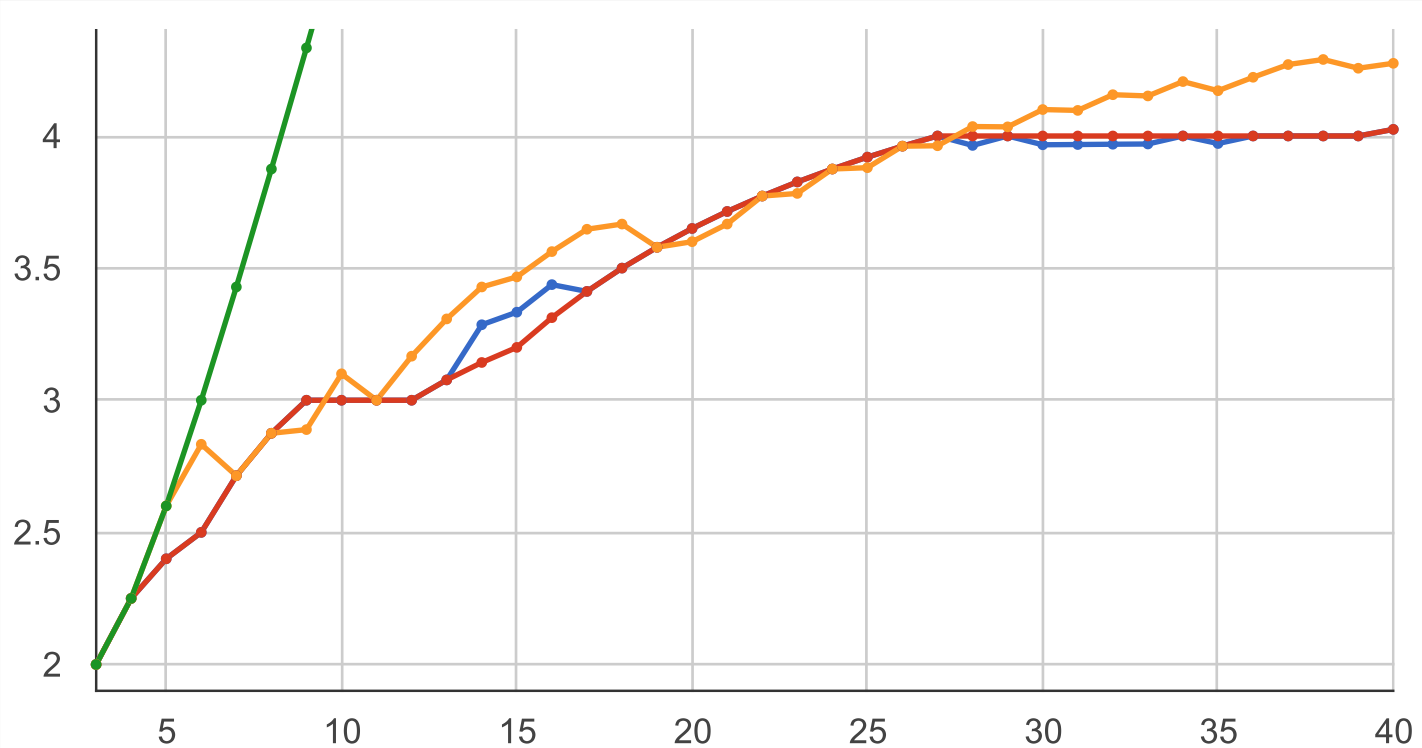
\includegraphics[width=4.5cm]{img-results.png}
        }{0.6}{0.4}
      \end{enumerate}
    \end{block}       
  \end{column}
  %%%%%%%%%%%%%%%%%%%%%%%%%%%%%%%%%%%%%%%%%%%%%%%%%%%%%%%%%%%%%%%%%%%%%%%%%%%%%%%%%%%%%%%%%%%%%%%%%%%%
  %%%%%%%%%%%%%%%%%%%%%%%%%%%%%%%%%%%%%%%%%%%%%%%%%%%%%%%%%%%%%%%%%%%%%%%%%%%%%%%%%%%%%%%%%%%%%%%%%%%%
\end{columns}
\vfill
\end{frame}

\end{document}
%%%%%%%%%%%%%%%%%%%% 
%%% Local Variables: 
%%% mode: latex 
%%% TeX-PDF-mode: t 
%%% End: 
